\section{暗物质晕的形成}

暗物质晕的形成也是 bottom-up scenario.
暗物质晕由小质量的晕通过并合逐渐增大的过程叫做 
Merger Tree. 如 \reffig{fig:MegerTree} 所示。

\begin{figure}[!hbtp]
	\centering 
	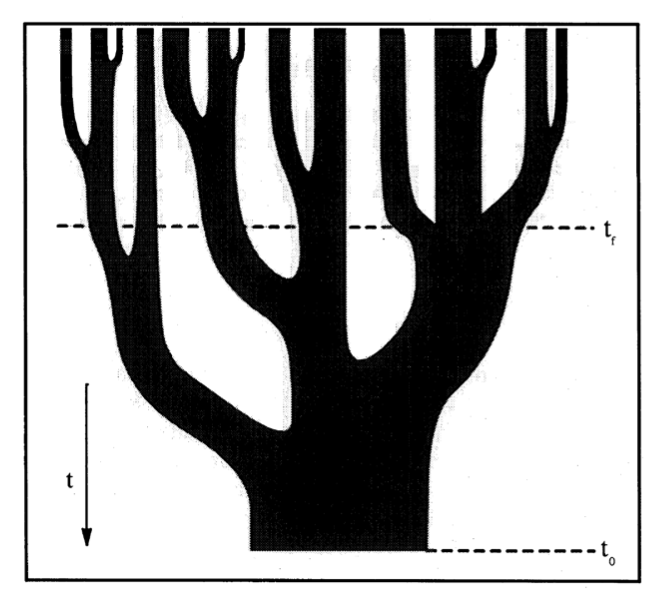
\includegraphics[width=1.0\linewidth]{MegerTree.png}
	\caption{Meger Tree 示意图}
    \label{fig:MegerTree}
\end{figure}

并合的过程也叫做 assembly history ,
assembly history 会影响 暗物质晕的性质,因此是目前重要的研究方向之一。

在暗物质晕的形成中,我们关心不同质量的暗物质晕分别会形成多少。
一个近似的方法是
随机行走 (Random Walk) of dark matter halo statistics.
物质密度的空间分布是随机的,当局部密度大于 临界密度 $\delta_\text{crit}$ 时,我们认为这里形成一个 暗物质晕。 如 \reffig{fig:RandomWalk} 所示,红色标出的区域是大小不同的暗物质晕。

\begin{figure}[!hbtp]
	\centering 
	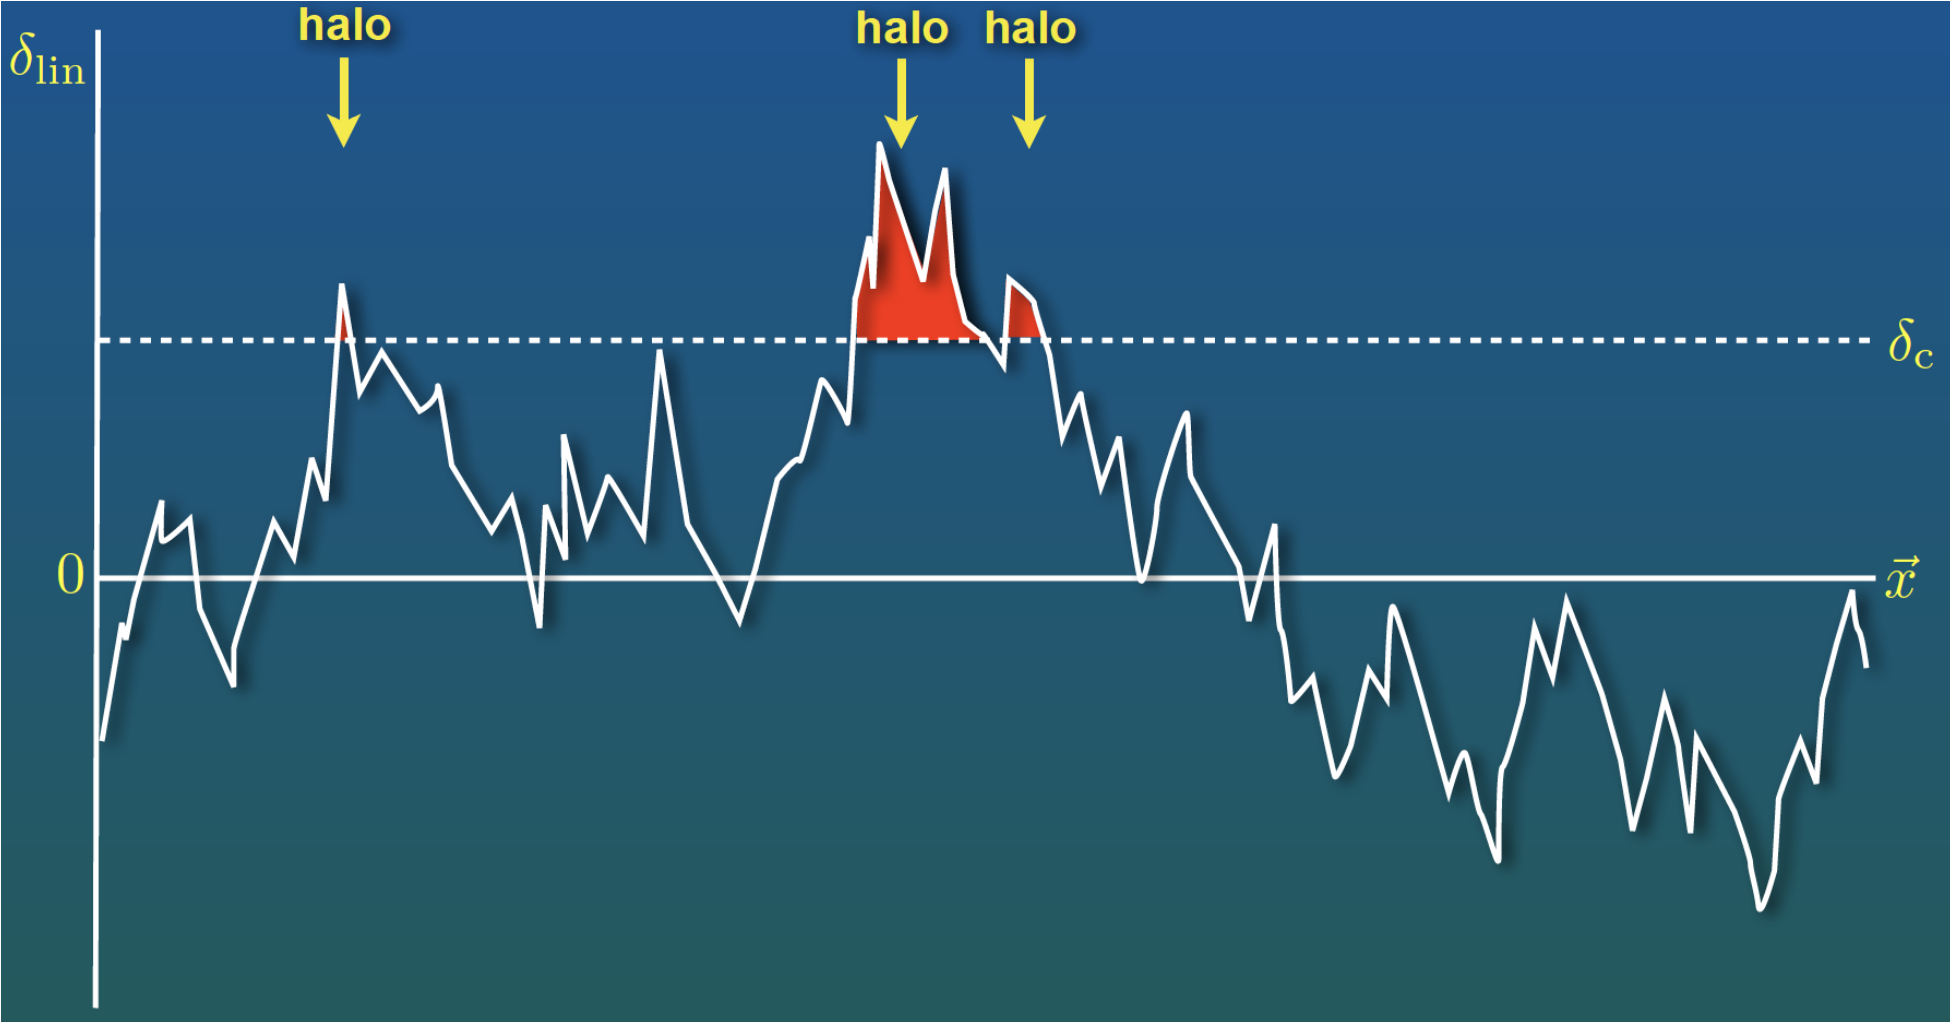
\includegraphics[width=1.0\linewidth]{Peaks_halo.png}
	\caption{Random Walk 示意图}
    \label{fig:RandomWalk}
\end{figure}

在 半径 $R$ 的范围内 对密度涨落做平滑: 
$\delta_M = \delta\left(\vec{x},R\right) $. 
这个平滑尺度对应 质量 $M=\bar{\rho} \times \frac{4}{3} \pi R^3$.

我们想计算 的 halo mass function 是 在一定质量范围内(大于$M$) halo 的数密度,
它 等于
在平滑尺度为 $M$ 时的  峰的 数密度
$n\left(>M\right) = n _{\rm{pk}} \left(\delta_M\right)$ .

Press-Schechter 模型
假设密度场是高斯分布
\begin{eqnarray}
    \mathcal{P}\left(\delta_{M}>\delta_{c}(t)\right) &=& F(>M, t) \\ 
    &=& \frac{1}{\sqrt{2 \pi} \sigma_{M}} \int_{\delta_{c}}^{\infty} \exp \left[-\frac{\delta_{M}^{2}}{2 \sigma_{M}^{2}}\right] d \delta_{M}=\frac{1}{2} \operatorname{erfc}\left[\frac{\delta_{c}}{2 \sigma_{M}}\right]
\end{eqnarray}
其中 $\operatorname{erfc}(x)=1-\operatorname{erf}(x)$, $\operatorname{erf}(x)=\frac{2}{\sqrt{\pi}} \int_{0}^{x} e^{-t^{2}} d t$ 是  error function.